\section{Introduction}
\label{sec:introduction}

\par The objective of this laboratory assignment is to design and study a AC-DC converter. We will choose and implement the architecture of the converter in a way that maximizes the figure of merit, according to equation [X].

\begin{equation}
    M = \frac{1}{cost \times (ripple(v_0) + average (v_0 - 12) + 10^6}
    \label{eq:v_s}
\end{equation}

The circuit to be analysed is presented in figure [XX]. It receives a AC input signal (230$V$/50$Hz$) and it's composed of a transformer with [NN] to 1 voltage ratio and galvanic isolation, followed by a Envelope Detector (ED) circuit and a Voltage Regulator (VR) circuit. The ideal output of the circuit is a 12$V$ DC signal. 

\par The ED and VR circuits are the ones to be freely designed.   
[composition of these circuits]

The results of the theoretical analysis will be compared with a computational simulation. The designed circuit can be seen in Figure \ref{fig:circuit}.

[IMAGEM DO CIRCUITO]
%\begin{figure}[H]   
%\centering
%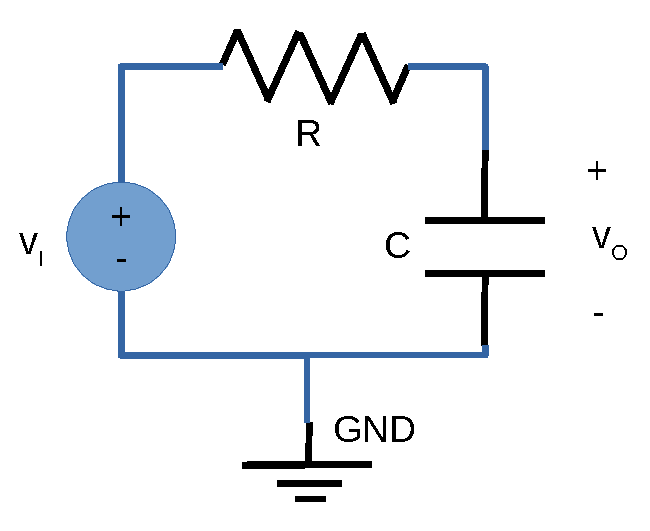
\includegraphics[width=10 cm]{rc.pdf}
%\caption{RC circuit to be studied}
%\label{fig:circuit}
%\end{figure}


\par In Section~\ref{sec:theoretical}, a theoretical analysis of the implemented circuit is presented, with the help of \textit{Octave} software. In Section~\ref{sec:simulation}, the circuit is analysed by simulation, using the software \textit{ngspice}, and the results are compared to the theoretical results obtained in Section~\ref{sec:theoretical}. The conclusions of this study are outlined in Section~\ref{sec:conclusion}.